\documentclass{article}

\usepackage{graphicx}
\usepackage{float}
\usepackage{cite}
\usepackage{url}

\begin{document}

\section{Basic Camera Model}

The basic camera model is implemented inside the camera class. The camera class
allows the creation of rays for a given pixel. The class first uses the Up and
Lookat vectors to create an orthogonal basis w, u, v. An field of view is defined
and then used along with the value for the width, hight and current pixel location
to calculate the point on the camera screen that corresponds to the top left corner
of the pixel. Once we have the point on the screen the viewing ray can be calculated
and returned.\\

In order to implement anti-aliasing for each pixel 16 rays, these are aranged in
a regular grid across the pixel where each ray is 0.25 pixel widths from the previous.
The colour values for each of these rays are then averaged to give the anti-aliased
value. Figure \ref{fig:antialias} shows a raytraced sphere with and without anti-aliasing
turned on.\\

\begin{figure}[H]
  \begin{center}
  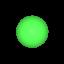
\includegraphics[width=150px]{Images/antialiasOff.png}
  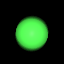
\includegraphics[width=150px]{Images/antialiasOn.png}
  \caption{Sphere raytraced with and without anti-aliasing}
  \label{fig:antialias}
  \end{center}
\end{figure}

\section{Plane \& Triangle Intersection}

The triangle intersection is done in the triangle class. The class takes three
vertexs as parameters, these are the three corners of the triangle. This first step in the
intersection test is to calculate the three vectors which make up the sides
of the triangle, these are used to get the normal by the application of the
cross product \cite{triabgle}. Using the normal and a point the intersection between the
ray and the plane the triangle lies on can be calculated then the value of t that
the ray intersects at can be found. After this the cross product is used to check
the intersection point is on the inside of each of the sides of the triangle.

\begin{figure}[H]
  \begin{center}
  
\includegraphics[width=150px]{Images/triangle.png}
  \caption{Triangle intersection}
  \label{fig:triint}
  \end{center}
\end{figure}

\section{Quadratic Intersection}

Quadratic surfaces are defined by 9 terms A - J in the equation below.

\begin{center}
$Ax^2 + 2Bxy + 2Cxz + 2Dx + Ey^2 + 2Fyz + 2Gy + Hz^2 + Iz + J = 0$
\end{center}

In order to calculate the intersection point between a ray and the surface the
ray equation $Dt + P = 0$ can be substituted into the quadratic. This substitution gives the
quadratic equation below where dx, dy and dz are the x,y and z components of the
direction and px, py and pz are the components of the initial ray position \cite{quadratic}.

\begin{center}
$Aqt^2 + Bqt + Cq = 0$ Where
$Aq = Adx^2 + Edy^2 + Hdz^2 + Bdxdy + Cdxdz + Fdydz$
$Bq = 2Apxdx + 2Epydy + 2Hpzdz + B(pxdy + pydx) + C(pxdz + pzdx) + F(pydz + pzdy) + Ddx + Gdy + Idz$
$Cq = Apx^2 + Epy^2 + Hpz^2 + Bpxpy + Cpxpz + Fpypz + Dpx + Gpy + Ipz + J$
\end{center}

This can then be solved using the quadratic equation, if there are no solutions
then the ray does not intersect the quadratic surface.

\begin{figure}[H]
  \begin{center}
  
\includegraphics[width=150px]{Images/quadCylinder.png}
  \caption{Quadratic Intersection}
  \label{fig:quadint}
  \end{center}
\end{figure}

\begin{figure}[H]
  \begin{center}
  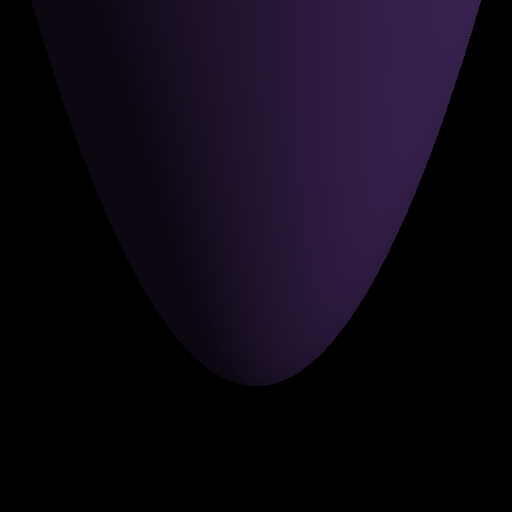
\includegraphics[width=150px]{Images/quadParaboid.png}
  \caption{Basic Camera Model}
  \label{fig:basiccammod}
  \end{center}
\end{figure}

\begin{figure}[H]
  \begin{center}
  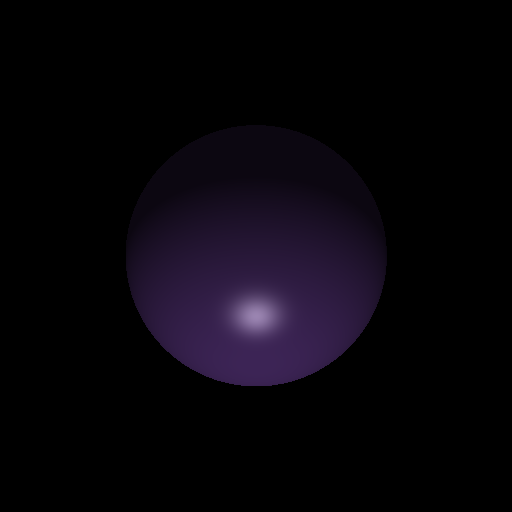
\includegraphics[width=150px]{Images/quadSphere.png}
  \caption{Basic Camera Model}
  \label{fig:basiccammod}
  \end{center}
\end{figure}

\section{Point Lights}



\begin{figure}[H]
  \begin{center}
  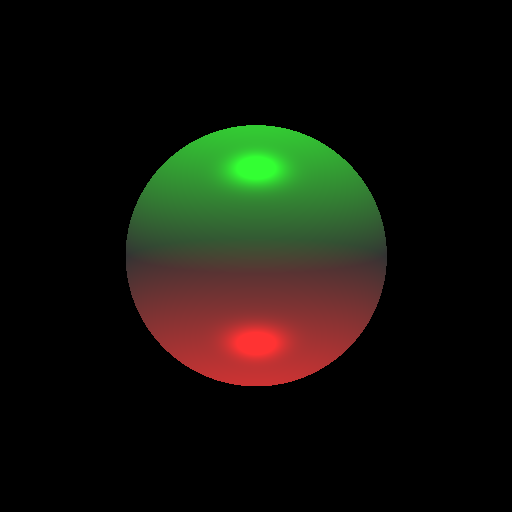
\includegraphics[width=150px]{Images/pointLight.png}
  \caption{Basic Camera Model}
  \label{fig:basiccammod}
  \end{center}
\end{figure}

\section{Specular Material}

\begin{figure}[H]
  \begin{center}
  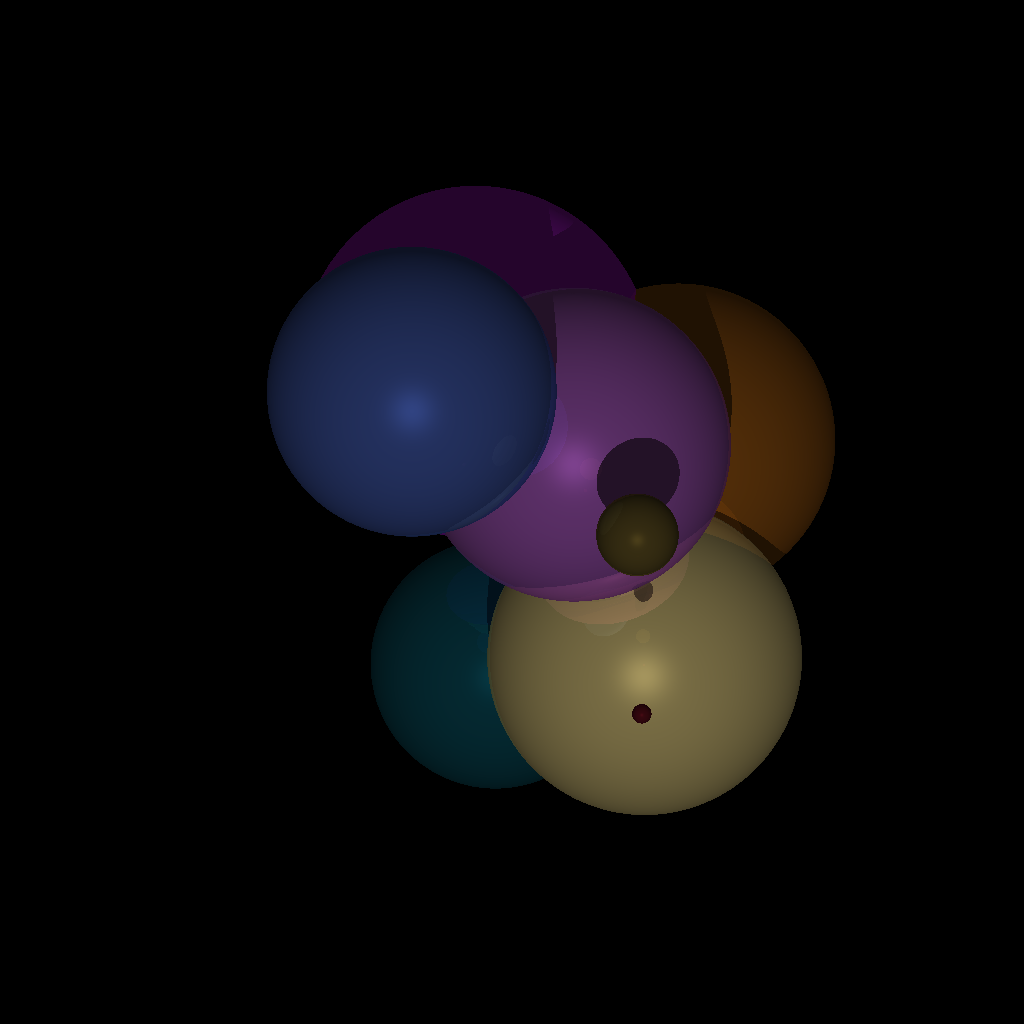
\includegraphics[width=150px]{Images/reflectionsOn.png}
  \caption{Basic Camera Model}
  \label{fig:basiccammod}
  \end{center}
\end{figure}
0.
\begin{figure}[H]
  \begin{center}
  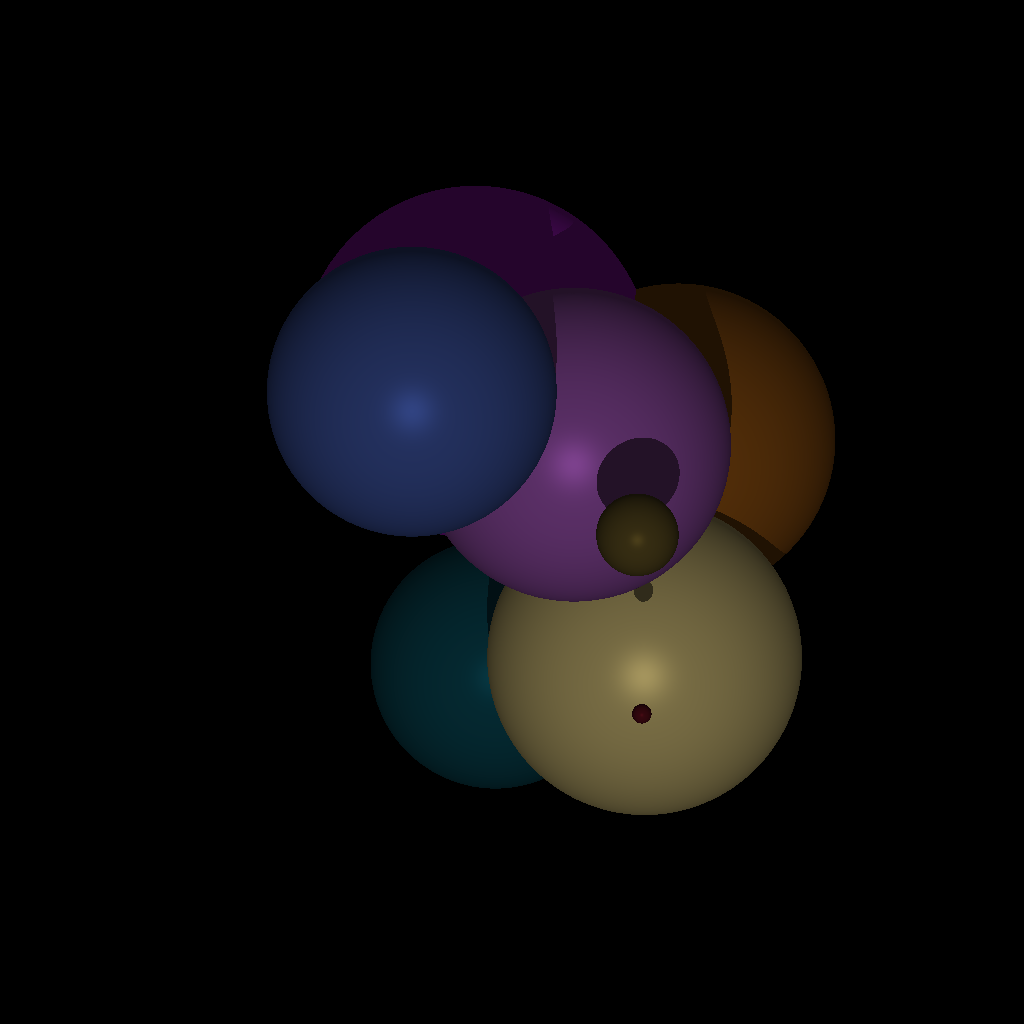
\includegraphics[width=150px]{Images/reflectionsOff.png}
  \caption{Basic Camera Model}
  \label{fig:basiccammod}
  \end{center}
\end{figure}

\begin{figure}[H]
  \begin{center}
  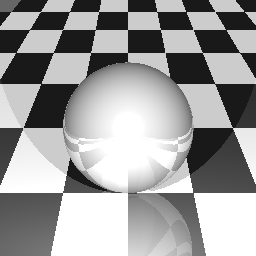
\includegraphics[width=150px]{Images/gridSphere.png}
  \caption{Basic Camera Model}
  \label{fig:basiccammod}
  \end{center}
\end{figure}

\section{Shadows}

\begin{figure}[H]
  \begin{center}
  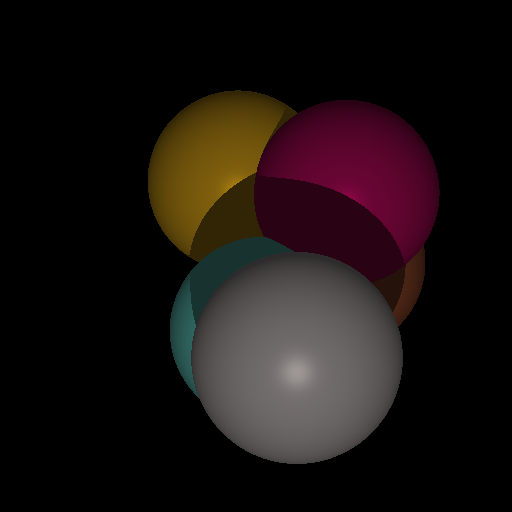
\includegraphics[width=150px]{Images/shadows.png}
  \caption{Basic Camera Model}
  \label{fig:basiccammod}
  \end{center}
\end{figure}

\section{Transparent Material}

\section{Octree}

\begin{figure}[H]
  \begin{center}
  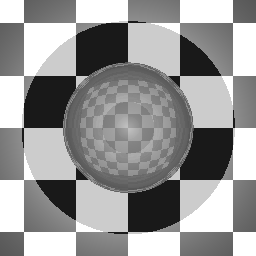
\includegraphics[width=150px]{Images/octreeTest.png}
  \caption{Basic Camera Model}
  \label{fig:basiccammod}
  \end{center}
\end{figure}

9 seconds with octree, 53 without.

\bibliographystyle{unsrt}
\bibliography{ref}

\end{document}